\documentclass{article}
\usepackage[T1]{fontenc}
\usepackage{lmodern}
\usepackage{graphicx}
\usepackage{amsmath,amssymb}
\usepackage[a4paper,margin=2cm]{geometry}
\usepackage[absolute,overlay]{textpos}
\setlength{\TPHorizModule}{1mm}
\setlength{\TPVertModule}{1mm}
\usepackage[indonesian]{babel}
\usepackage{hyperref}
\setlength{\emergencystretch}{2em}
% unit: Halaman 39

\begin{document}

% === Halaman 39 (llm) ===

% (tidak ada teks dari model)

% deskripsi: Diagram proses enkripsi dan dekripsi simetris yang menunjukkan aliran pesan dari plainteks 'Kirim senjata perang P', melalui proses Enkripsi $E_K(P) = C$ dengan kunci 'ocean' menjadi cipherteks 'Stype xouvatx kutreq C', lalu proses Dekripsi $D_K(C) = P$ dengan kunci yang sama kembali menjadi plainteks 'Kirim senjata perang P'.
% bbox normalisasi: [0.0700, 0.3020, 0.9320, 0.6530]
\begin{textblock*}{181.02mm}(14.70mm,89.69mm)
\noindent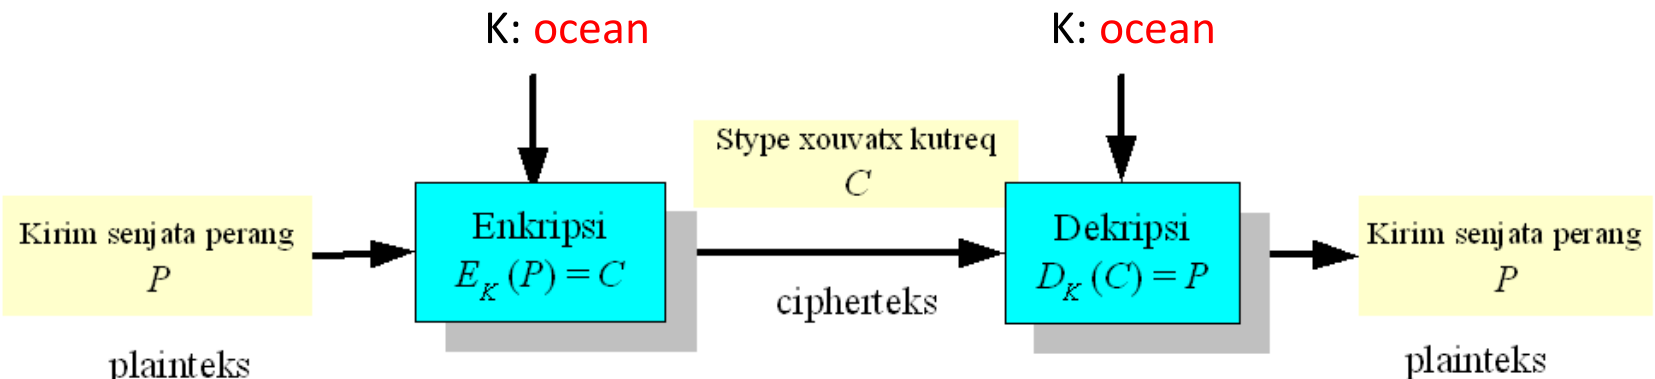
\includegraphics[width=181.02mm,height=104.25mm]{../../images/llm/page_039_img_01.png}%
\end{textblock*}

\end{document}
